\section{Experimental Results}
\label{sec:exp}
{\color{red}We evaluate our algorithm on three datasets: synthetic XOR datasets, the Omniglot low-shot benchmark and the large-scale ImageNet dataset. We use our own implementation of SGM approach \cite{low-shot} for a fair comparison.}

%The Omniglot dataset consists of over 1600 separate classes with only a few examples per class, aptly lending to it being called the transpose of MNIST (Lake et al., 2015).
\subsection{Synthetic Datasets}
\begin{figure}
	\begin{center}
	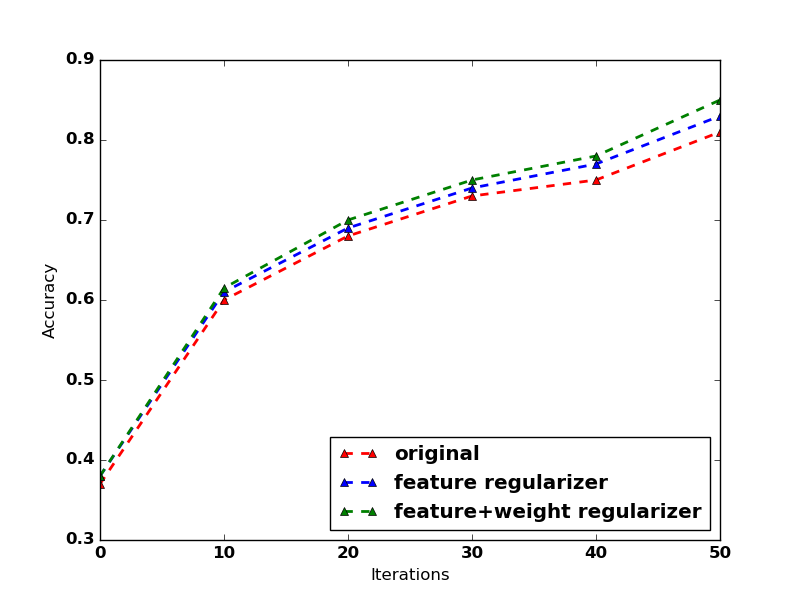
\includegraphics[width=0.5\columnwidth]{xor-plot.png}
	\end{center}
	%
	%	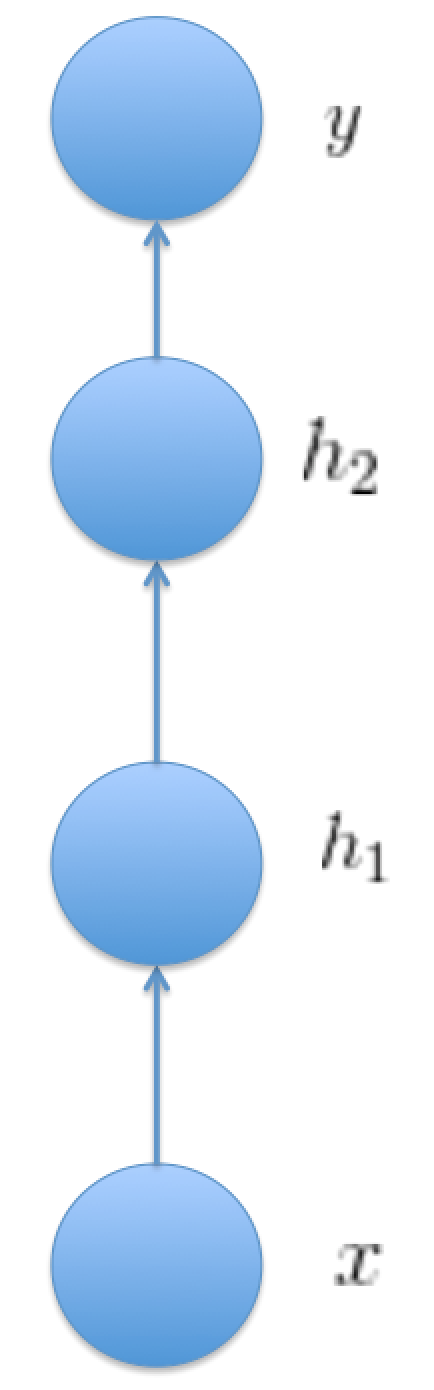
\includegraphics[width=0.3\columnwidth]{xor.png}\hspace{+0.5mm}
	%	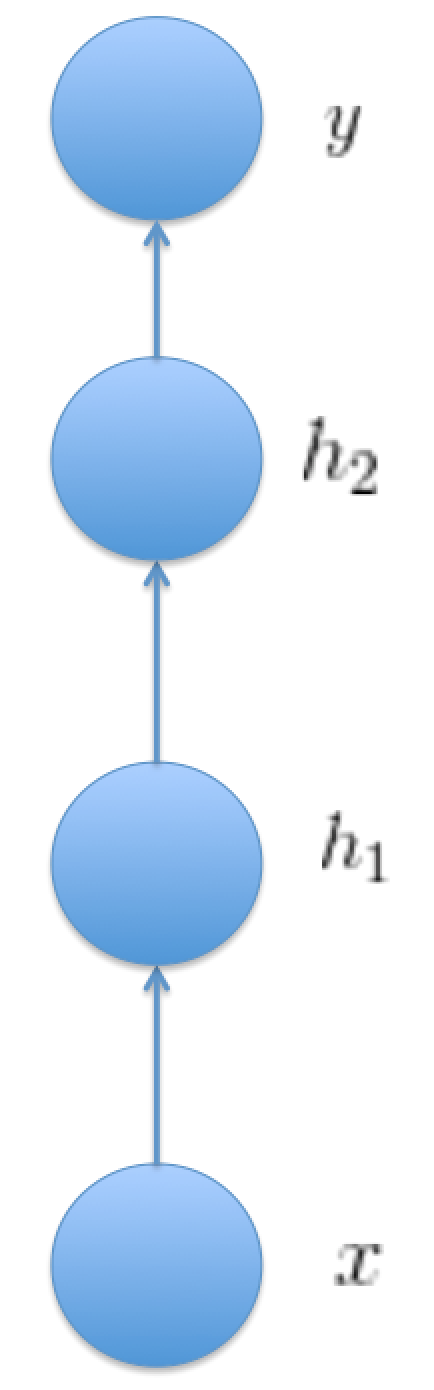
\includegraphics[width=0.3\columnwidth]{xor.png}\vspace{+1mm}\\
	%
	%\hspace{+0mm}
	%\vspace{-2mm}
	\caption{Evaluation on the XOR classification task. The red, blue and green lines stand for the accuracy of the Neural Network without any regularization, only the $L_2$ feature penalty, and our model with both weight and feature regularizer, respectively.}
	\label{fig-xor-plot}
\end{figure}
We first evaluate our model on the XOR dataset. Without loss of generality, we assume the data points $\mathbf{x}=[x_1,x_2]^T$ are uniformly sampled from a rectangle $x_1\in [-1,1],x_2\in [-1,1]$, and $y(\mathbf{x})=\mathbb{I}(x_1*x_2>0)$. The structure we use is a two-layer non-linear neural network with one latent layer $h=\sigma(W_1\mathbf{x}+\mathbf{b})$ where $\sigma(.)$ is the rectified linear unit. ADAM \cite{adam} is leveraged to numerically optimize the cross entropy loss.

During training, we make use of only 4 points $\{[1,1],[-1,1],[1,-1],[-1,-1]\}$, while randomly sampled points from the whole rectangle as the test set. It is a very low-shot task. As shown in Figure \ref{fig-xor-plot}, our model with both feature and weight regularization outperforms the gradient penalty \cite{low-shot} and no regularization. We use uniform feature penalty as in Eqn(\ref{eqn:final-cost}) and set $\lambda_1=\lambda_2=0.1$ in our experiments.

\subsection{Low-shot learning on Omniglot}
Our second experiment is carried out on the Omniglot one-shot benchmark \cite{lake-omniglot}. Omniglot training set contains 964 characters from different alphabets with only 20 examples per each character. The one-shot evaluation is a pairwise matching task on completely unseen alphabets.

Following \cite{matching-network}, we use a simple yet powerful CNN as feature representation model, consisting of a stack of modules, each of which is a $3\times3$ convolution with $128$ filters followed by batch normalization\cite{batch-normalization}, a ReLU and $2\times2$ max-pooling. We resized all images to $28 \times28$ so that the resulting feature shape satisfies $\phi(x)\in\mathbb{R}^{128}$. A fully connected layer followed by a softmax non-linearity is used to define the Baseline Classifier.

We set $\lambda_1$=1e-4 in SGM \cite{low-shot} and $\lambda_1$=$\lambda_2$=1e-4 in our model. A nearest neighbor approach with $L_2$ distance of feature $\phi(\mathbf{x})$ is applied for one-shot evaluation. As shown in Table 1, we can see that our model with both feature and weight penalty is able to achieve satisfactory performance of one-shot $91.5\%$ accuracy, highly competitive with the state-of-the-art Matching Network\cite{matching-network} with CNN warm-start and RNN hyper-parameter tuning.

\begin{table}
\center
\begin{small}
	\renewcommand{\arraystretch}{1.1}
	\begin{tabular}{c|c}
	\hline
	Model & One-shot Evaluation \\
	\hline
	Random Guess & 5\%\\
	Pixel-KNN & 26.7\%\\
	MANN \cite{mann} & 36.4\%\\
	CNN Metric Learning & 72.9\% \\
	\hline
	CNN (Our implementation) & 85.0\% \\
	Low-shot \cite{low-shot} & 89.5\% \\
	{\color{red} Matching Network \cite{matching-network}} & {\color{red}93.8\%} \\
	\textbf{Ours} & \textbf{91.5\%}\\
	\hline
	\end{tabular}
	\caption{Experimental results of our algorithm on the Omniglot benchmark \cite{lake-omniglot}. }
	\end{small}
\label{tab:omniglot}
\end{table}

\subsection{Large-scale Low-shot Learning on ImageNet}
Our last experiment is on the ImageNet benchmark \cite{russakovsky2015imagenet}. It contains a wide array of classes with significant intra-class variation. We divide the 1000 categories randomly into 400 base for training and evaluate our feature representation on the 600 novel categories. 

We use a 50-layer residual network \cite{residual_net} as our baseline. Evaluation is measured by top-1 accuracy on the 600 test-set in a 20-way setup, i.e., we randomly choose 1 sample from 20 test classes, and applies a nearest neighbor matching.
As shown in Table 2, %\ref{tab:imagenet},
we can see that our model learns meaningful representations for unseen novel categories even with large intra-class variance.
\begin{table}
\center
\begin{small}
\renewcommand{\arraystretch}{1.1}
\begin{tabular}{c|c}
\hline
Model & One-shot Evaluation \\
\hline
CNN baseline & 40.1\%\\
Low shot \cite{low-shot} & 46.0\% \\
\textbf{Ours} & \textbf{46.6\%}\\
\hline
\end{tabular}
\caption{Experimental results of our algorithm on the ImageNet benchmark \cite{russakovsky2015imagenet} with the 20-way one-shot setting. }
\end{small}
\label{tab:imagenet}
\end{table}

{\color{red}\subsection{Comparison with Batch-Normalization}}
\begin{figure}
\begin{center}
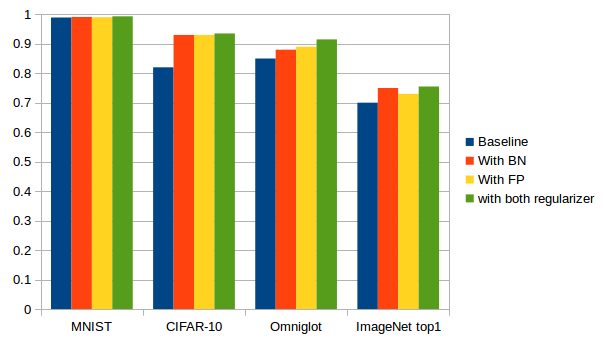
\includegraphics[width=0.6\columnwidth]{classification.png}
\end{center}
\caption{{\color{red}Classification accuracy comparison of our feature penalty (termed ``PN'') with batch-normalization (termed ``BN'') \cite{batch-normalization} on MNIST, CIFAR-10, Omniglot and ImageNet benchmarks. We compare baseline methods with neither batch-normalization nor feature penalty, with each module added, and with modules included.}}
\label{fig-compare-bn}
\end{figure}
{\color{red}As discussed in Section 2.3, feature penalty has similar effects with batch normalization \cite{batch-normalization}. It is of interest to compare the influence of two modules influence training performance of neural networks. We study the performance of the classification with and without each modules on four classic image classification benchmarks. For CIFAR-10 and ImageNet, we applied the Residual Net architecture \cite{residual_net}, while stacked convolution layers with ReLU and max-pooling is applied for MNIST and Omniglot. For ImageNet benchmark evaluation, we test the top-1 accuracy on the validation set with 50,000 images.
	
Since in our model the feature penalty regularizer is applied only on the last hidden layer, we still keep the batch-normalization modules in previous layers in our ``FP'' model. As shown in Figure \ref{fig-compare-bn}, we observe that baseline models with neither ``BN'' nor ``FP'' takes much longer to converge and achieve inferior performance; our ``FP'' regularizer achieves almost the same performance on MNIST (both 99\%), CIFAR-10 (both 93\%) and Omniglot 1-shot (88\% BN v.s. 89\% FP); on ImageNet, ``BN'' performs better than our ``FP'' (75\% BN v.s. 74\% FP). With both batch-normalization and feature penalty modules added, we achieve the best classification performance on all four benchmarks.
}